%! TEX root = ../000-main.tex

\section[Study of Accuracy]{Study of Accuracy for large problems}

\subsection{Experiment setup}

We'll study the accuracy of the three algorithms. To do so, we
repeat the experiments of \cref{sub:convergence_setup} but this time
we'll use a more realistic dataset, generated from the following
parameters:
\begin{center}
    \begin{BVerbatim}
    tr_p = 20000; te_q = tr_p/10; tr_freq = 0.0;
    \end{BVerbatim}
\end{center}

The main differences are that now, we have a much larger training and test
sets and that the training set is now balanced, meaning that it has the same
number of samples from each class.

We'll use the values of $\lambda$ that gave the best accuracy in
the experiments from~\cref{sec:convergence} for each algorithm.
These previous results are shown in~\cref{tab:te_acc_250}.

\begin{table}[ht]
    \caption{Accuracy on test set from previous experiment (\texttt{tr\_p = 250}) with
    the highest average accuracy for each method in bold}%
    \label{tab:te_acc_250}%
    \begin{talltblr}{
	colspec={cS[table-format=1.2]S[table-format=2.1(1)]}
	}
	\toprule
	Algorithm & {{{$\lambda$}}} & {{{$Accuracy^{TE}\pm \sigma$}}} \\ \midrule
	GM        & 0               & 99.2(9)                         \\
	QNM       & 0               & 99.4(7)                         \\
	\SetRow{bg=gray9,font=\bfseries}
	SGM       & 0               & 99.6(5)                         \\
	\addlinespace
	\SetRow{bg=gray9,font=\bfseries}
	GM        & 0.01            & 99.5(8)                         \\
	\SetRow{bg=gray9,font=\bfseries}
	QNM       & 0.01            & 99.5(8)                         \\
	SGM       & 0.01            & 99.4(5)                         \\
	\addlinespace
	GM        & 0.1             & 97(5)                           \\
	QNM       & 0.1             & 97(5)                           \\
	SGM       & 0.1             & 94(4)                           \\ \bottomrule
\end{talltblr}

\end{table}

\pagebreak
% \subsection{Results}

% For this analysis, our main focus is on the accuracy obtained on the test set and
% the time it takes to obtain it.

\subsection{Accuracy}

Let's start by looking at the accuracy obtained from the three algorithms
taking into account the different values of $\lambda$. The results are shown in
\cref{fig:lambda_acc_2}. We can see that the accuracy values obtained from the
train and test sets are very similar, which is a good sign that the model is
not overfitting. Moreover, the accuracy values for each method are very similar
to each other (except some outliers on $QNM$ with $\lambda = 0$). Which would
suggest that the three methods are equally good at finding the optimal solution
when using the same regularization parameter.

\begin{figure}[H]
    \input{../analysis/acc_lambda_acc.tikz}
    \caption{Accuracy on train and test set for all algorithms with different values of $\lambda$}
    \label{fig:lambda_acc_2}
\end{figure}

Given that the accuracy of $\lambda=0.1$ is notably lower than the rest it
makes it difficult to distinguish the differences from the other values.
Any accuracy lower than 90\% given the proportion of the samples is no better
than classifying everything as a non-match.
% Therefore, the values obtained with $\lambda=0.1$ are not considered in the following analysis.
In fact, if we look at the results for one of the instances with accuracy 89.95\%,
we can see that everything is a false negative as illustrated in \cref{fig:fneg} where
we can see that everything is classified as not a 3.

\begin{figure}[H]
    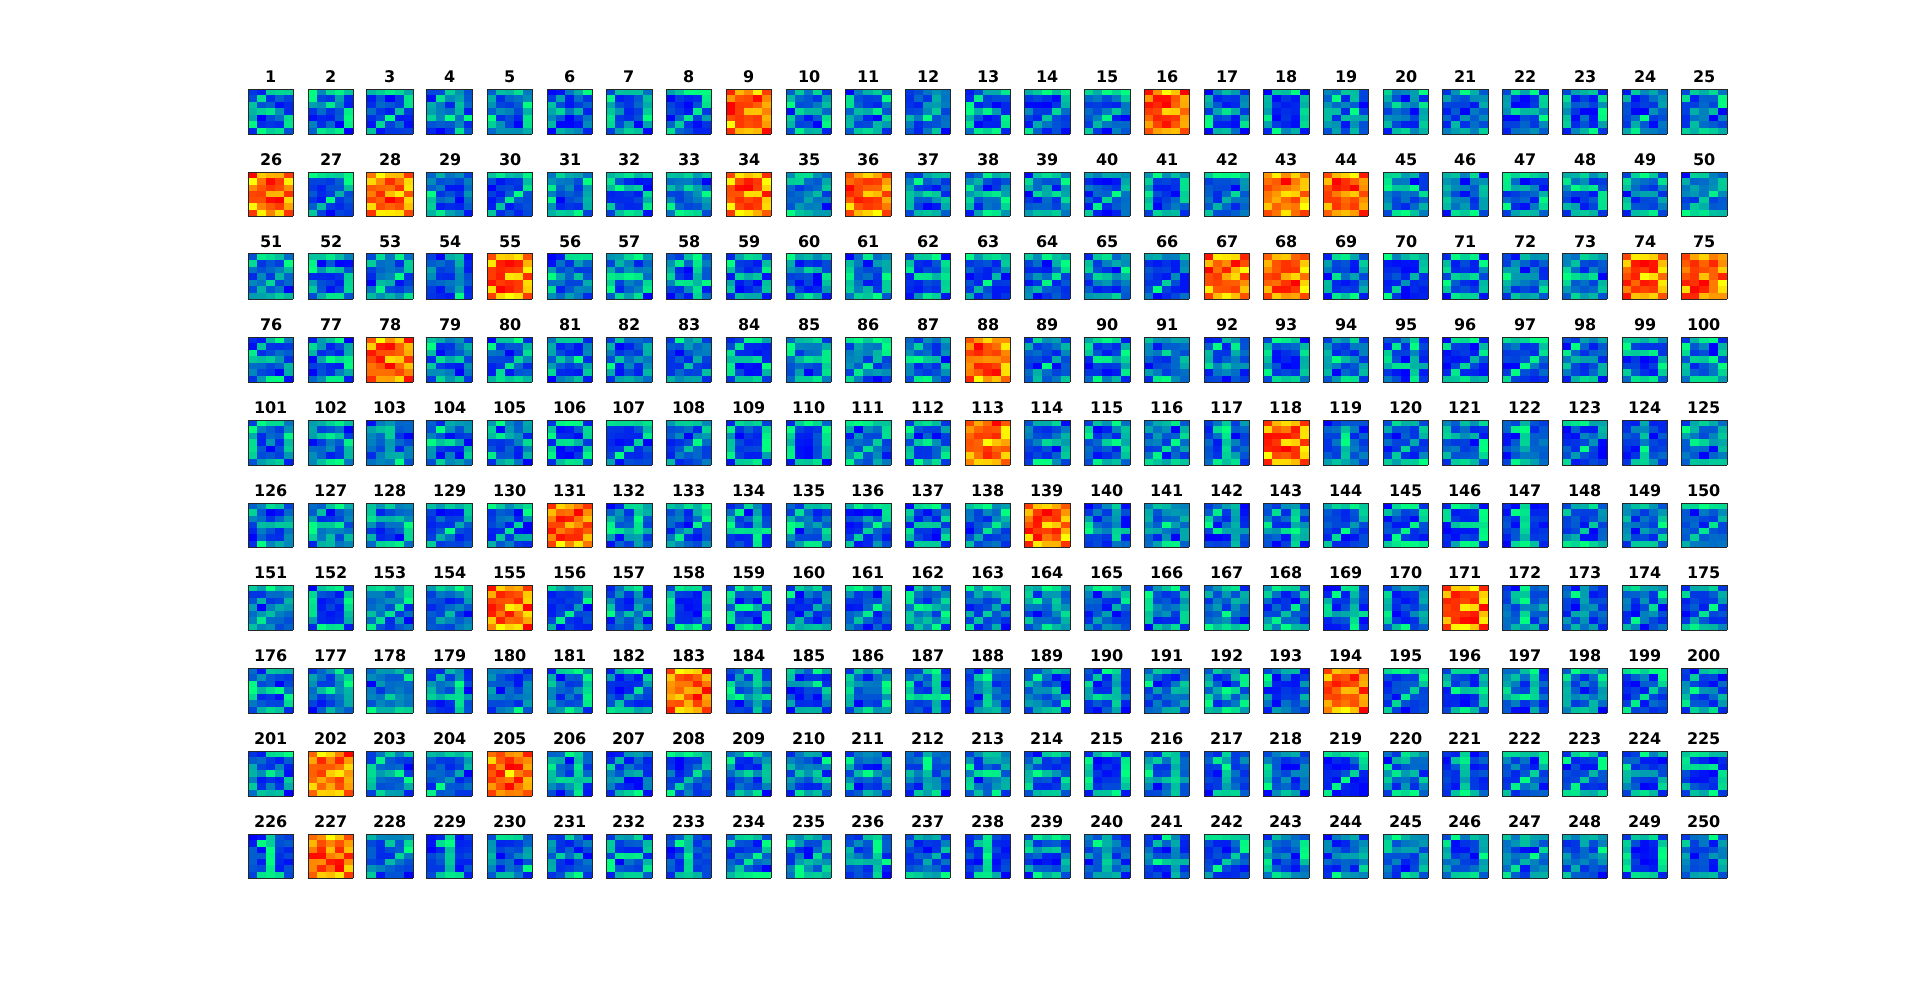
\includegraphics[width=\textwidth]{../src/SGM_te_plot_2k_01.png}
    \caption{Sample of first 250 from test set of $SGM$ with $\lambda=0.1$ and target 3,
    false negatives are shown in red and true negatives in blue}
    \label{fig:fneg}
\end{figure}

For reference, \cref{fig:fneg-001} shows the same sample but with $\lambda=0.01$, where
we can see that now there are true positives (in green) and much fewer false negatives.
The accuracy in this case is 97.95\%. There are no false positives (pink) in this particular
sample.

\begin{figure}[H]
    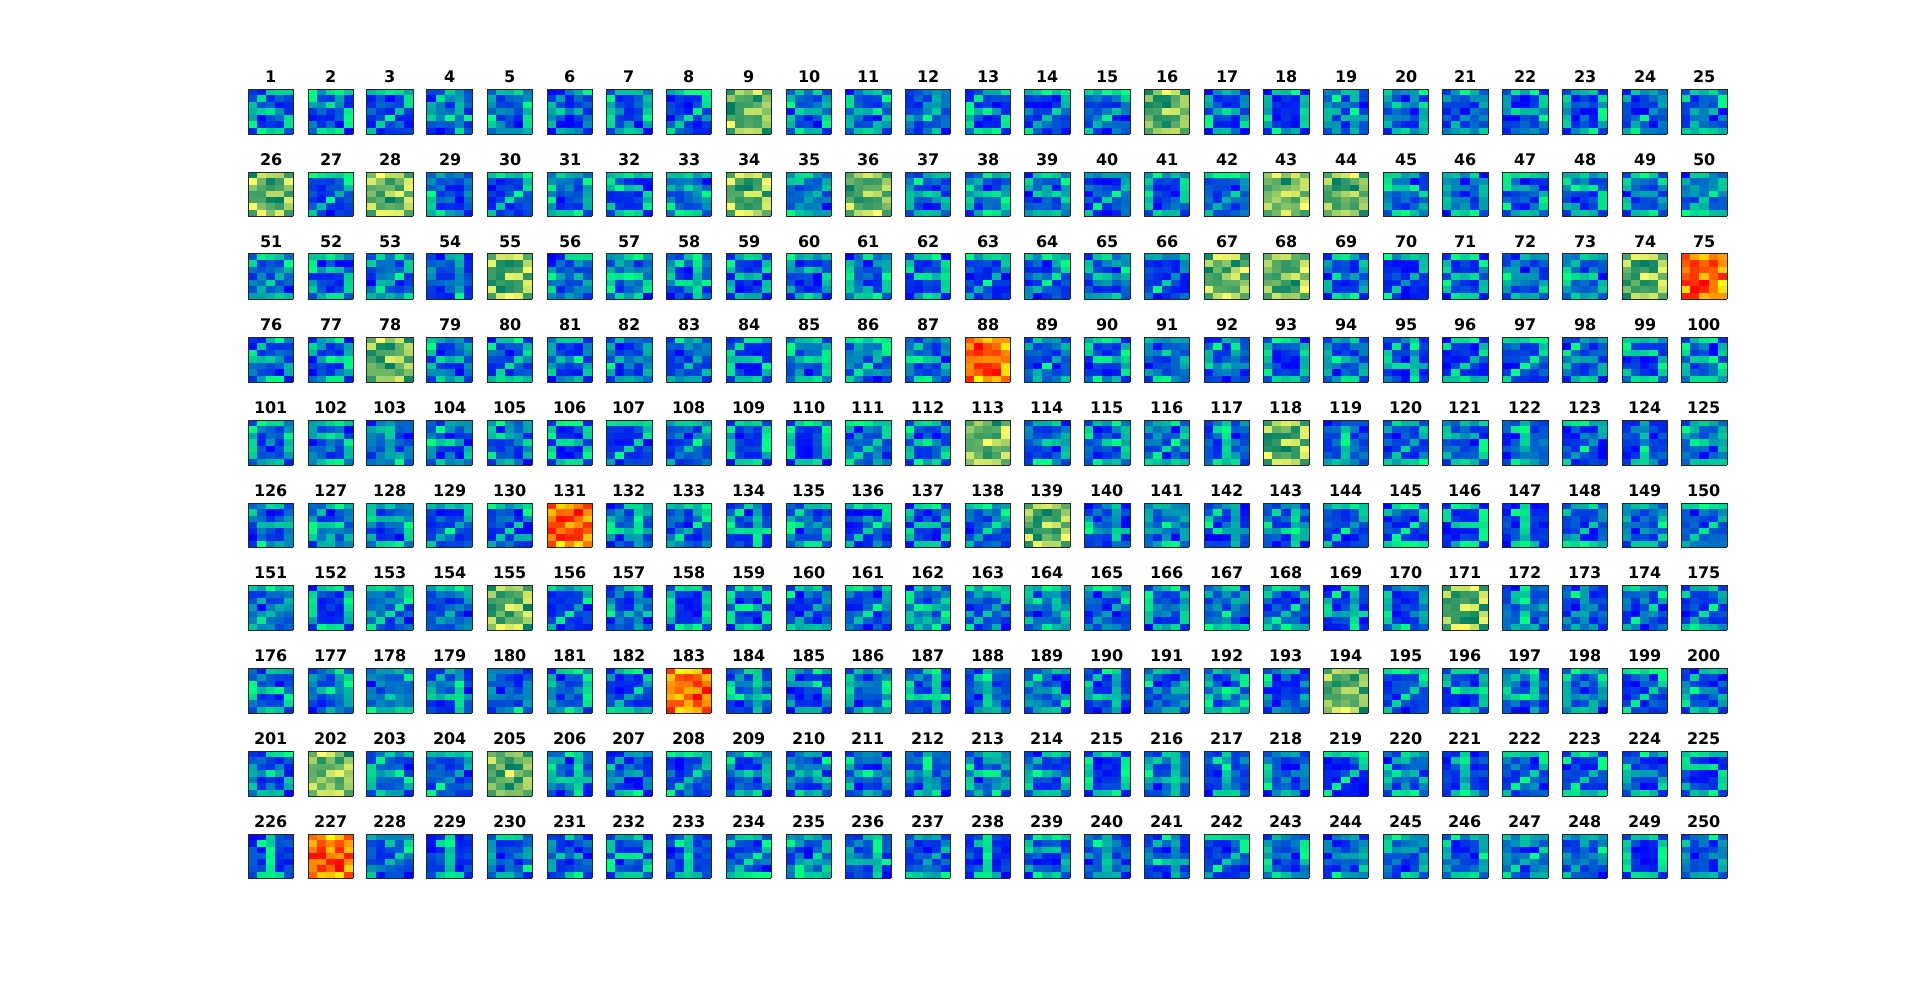
\includegraphics[width=\textwidth]{../src/SGM_te_plot_2k_001.png}
    \caption{Sample of first 250 from test set of $SGM$ with $\lambda=0.01$ and target 3,
    false negatives are shown in red, true negatives in blue and true positives in green}
    \label{fig:fneg-001}
\end{figure}

\pagebreak
Let's now look at the detail on the accuracy of the \emph{test} set for
$\lambda \neq 0.1$. This detailed magnification is shown in~\cref{fig:lambda_acc_2_detail}.
There, we can see that without regularization ($\lambda = 0$) the accuracy is
near 99.7\% for all three methods, while with $\lambda = 0.01$ the accuracy is slightly
lower, but still very high. Keep in mind that for $QNM$ we are omitting 2 outliers on
$\lambda = 0$ that are not shown in the figure. $SGM$ has slightly higher accuracy in
both cases.

\begin{figure}[H]
    \input{../analysis/acc_te_detail.tikz}
    \caption{Detail on the accuracy on test set for all algorithms for values of $\lambda \neq 0.1$ and
    omitting outliers}
    \label{fig:lambda_acc_2_detail}
\end{figure}

From \cref{fig:lambda_acc_2,fig:lambda_acc_2_detail} we can draw the following conclusions regarding
the accuracy of the three algorithms and the different values of $\lambda$:
\begin{enumerate}
    \item They all have very similar accuracy, however $SGM$ outperforms the other by a
        small margin.
    \item Without regularization we obtain very high accuracies, but we risk not reaching
        a proper solution (as is the case with the outliers in $QNM$ in our results).
\end{enumerate}

Therefore, in terms of accuracy, we can conclude that $SGM$ is the best method.

\pagebreak
\subsection{Training speed}

Let's now look at the training speed of the algorithms. We'll start by looking
at the time it takes to train the model for each value of $\lambda$ and
algorithm. The results are shown in~\cref{fig:lambda_time_2}. The time
is in logarithmic scale to better see the differences between the values.

From the figure, we can see that $SGM$ is the fastest method in all cases, by more
than an order of magnitude. This difference is even more noticeable when
we don't use regularization ($\lambda = 0$). In this case, $SGM$ takes
no more than 3 seconds (except for one outlier at 11), while the other
two take up to 100 seconds, and even the fastest outliers of
$QNM$ and $GM$ take more than 10 seconds.

\begin{figure}[H]
    \input{../analysis/acc_te_tex.tikz}
    \caption{Time to train the model for all algorithms with different values of $\lambda$}
    \label{fig:lambda_time_2}
\end{figure}

If we now look at the number of iterations%
\footnote{We use epochs instead of iterations for $SGM$ as explained in~\cref{ssub:epochs}.
In this case, ${e^{SG} = k^{SG}/100}$.}
instead of the execution time, we can see that the high execution times for
$QNM$ and $GM$ are due to the fact that they do not converge. Looking at
\cref{fig:lambda_nie_2} we can see that they reach
the maximum number of iterations set in the experiment (1000) in most cases
when $\lambda = 0$, to the point that the boxplot is a flat line at Iterations = 1000.
There is also an instance where $SGM$ reaches the maximum number of iterations.

\begin{figure}[H]
    \input{../analysis/acc_te_nie.tikz}
    \caption{Iterations to train the model for all algorithms with different values of $\lambda$}
    \label{fig:lambda_nie_2}
\end{figure}

From the results on execution time, there is a clear winner: $SGM$ is the fastest
method by far. Combining this with the fact that it also has the highest accuracy,
we can conclude that $SGM$ with $\lambda = 0.01$ is the algorithm and regularization
parameters from what we have tested. We cannot use $\lambda = 0$ as we have seen that
it can lead to non-convergence, which did not happen with our smaller dataset in the
first experiment but with this larger one we had one case.

\pagebreak
\subsection{Differences with previous experiment}

Now, we will compare the plots of execution time and iterations
from the first experiment (Experiment 1), with
the ones from this new one which has a bigger data size (Experiment 2). The aim of the comparison
is to quantify how the increase in size of the dataset
from 250 to $20\,000$ affects the performance of each algorithm.

\subsubsection{Iterations}

\Cref{fig:comp_niter} shows the comparison of the number
of iterations from both experiments. There are some notable differences:
\begin{enumerate}
    \item When $\lambda = 0$ in Experiment 2 we reach the maximum number of iterations
        before convergence in most cases, this is not the case in Experiment 1 where
        we have much more variability. This shows that regularization is important
        with bigger datasets.
    \item When $\lambda \neq 0$, the behaviour of both experiments is similar, with
        a slight increase in the number of iterations in Experiment 2, but not
        significant.
\end{enumerate}

\begin{figure}[H]
    \input{../analysis/comp_niter.tikz}
    \caption{Comparison of the number of iterations for the two experiments}
    \label{fig:comp_niter}
\end{figure}

\pagebreak
\subsubsection{Execution time per iteration}

\Cref{fig:comp_tex} shows the comparison of the execution time per iteration in the
two experiments. There is a clear difference in computation time between the two, but
we can see that a priori, the increase in execution time per iteration of
$SGM$ is smaller than the increase in execution time per iteration of $QNM$ and $GM$.

\begin{figure}[H]
    \input{../analysis/comp_tex.tikz}
    \caption{Comparison of the execution time per iteration for the two experiments}
    \label{fig:comp_tex}
\end{figure}

To quantify the increase in execution time per iteration, we can look at
\cref{fig:comp_ratio}. There, we can clearly see that indeed the increase
in execution time per iteration of $SGM$ is much smaller than the increase
in execution time per iteration of $QNM$ and $GM$. Keep in mind, that
the increase in data is 250 \textrightarrow{} $20\,000$, which is a factor of 80.
$GM$ and $QNM$ seem to have a linear increase in execution time per iteration,
while $SGM$ has sublinear increase.

\begin{figure}[H]
    \input{../analysis/acc_tnie_ratio.tikz}
    \caption{Comparison of the increase the execution time per iteration from one
    experiment to the other}
    \label{fig:comp_ratio}
\end{figure}

% \begin{figure}[H]
%     \input{../analysis/acc_tex_over_nie.tikz}
%     \caption{Time to train the model for all algorithms with different values of $\lambda$}
%     \label{fig:tex_over_nie2}
% \end{figure}

\subsection{Conclusions}

In the discussion of the previous experiment (\cref{ssub:discussion}) we concluded that
$SGM$ with $\lambda = 0.01$ was the best method for the minimization of
$\tilde L$. In this experiment, we have seen that again, $SGM$ with $\lambda = 0.01$
is the best method when aiming to maximize the accuracy on the test set.

The decision from the first experiment was opinionated since
$SGM$ did not give the lowest value of $\tilde L$, but it was small enough and
considerably faster than the others. In this experiment, $SGM$ outperforms the other
methods both in terms of accuracy and execution time. Not only that, but also, we have
seen that the increase in execution time per iteration of $SGM$ is much smaller than
the increase in execution time per iteration of $QNM$ and $GM$ in relation to the
increase in data size.

With our limited sample size,
we can conclude that for larger datasets,
$SGM$ is the best method to use by all accounts. We can also conclude that the value
of the regularization parameter $\lambda$ is really important and should be tuned
carefully. On one hand, if the value of $\lambda$ is too small, the algorithm can take a long time
to converge or exceed the maximum number of iterations. On the other hand, if the value
of $\lambda$ is too large, the algorithm can converge to a local minimum were all the results
are negative, which is undesirable.

